\section{Development Results and Pending Experiments}
\subsection{Preliminary Results Contract}
The separate non-CAMS run completed 24 temporal evaluations,
36 spatial holdouts and 12 calibration-window evaluations;
0 temporal and 0 spatial entries lacked sufficient data.
Its predictions and per-fold metrics come from the exact immutable artifact
recorded in the claim-evidence package. Strict Ridge had lower paired MAE than climatology (signed difference -8.96 AQI; 95\% date-block interval [-12.49, -5.61]; n=38382 exact pairs); lower MAE supported by this interval. History Ridge had higher paired MAE than persistence (signed difference +0.61 AQI; 95\% date-block interval [-0.41, +1.70]; n=31622 exact pairs); a nonzero MAE difference is not established by this interval.
These preliminary comparisons do not establish production approval. They do not answer
whether CAMS station correction improves a genuine operational baseline.
The definitive results table and skill figure remain:
[RESULT PENDING CAMS ARCHIVE EXPERIMENT]

% BEGIN PRELIMINARY FIGURE
\begin{figure}[h]\centering
\setlength{\unitlength}{1mm}
\begin{picture}(78,38)
\put(8,5){\line(1,0){64}}
\put(56,5){\line(0,1){26}}
\put(8.00,4){\line(0,1){2}}
\put(8.00,1){\makebox(0,0){\scriptsize -15}}
\put(24.00,4){\line(0,1){2}}
\put(24.00,1){\makebox(0,0){\scriptsize -10}}
\put(40.00,4){\line(0,1){2}}
\put(40.00,1){\makebox(0,0){\scriptsize -5}}
\put(56.00,4){\line(0,1){2}}
\put(56.00,1){\makebox(0,0){\scriptsize 0}}
\put(72.00,4){\line(0,1){2}}
\put(72.00,1){\makebox(0,0){\scriptsize 5}}
\put(16.04,26){\line(1,0){22.01}}
\put(27.33,26){\circle*{1.5}}
\put(40,31){\makebox(0,0){\scriptsize Strict Ridge minus climatology}}
\put(54.69,13){\line(1,0){6.76}}
\put(57.97,13){\circle*{1.5}}
\put(40,18){\makebox(0,0){\scriptsize History Ridge minus persistence}}
\end{picture}
\caption{NON-CAMS preliminary paired MAE differences and 95\% seven-day date-block intervals. Zero means equal MAE; lower is better. Strict $n=38,382$; history $n=31,622$.}
\end{figure}
% END PRELIMINARY FIGURE
% BEGIN PRELIM_SCOPE
\subsubsection{Limits of the preliminary experiment}
The non-CAMS plan uses 30 valid training days per station and a fixed Ridge
penalty of 10; these choices must not be mistaken for primary CAMS tuning.
The locked primary station rule remains 120 valid training days. Thus the
first 90-day primary training window cannot meet station eligibility; it
must be reported as insufficient, not rescued by future coverage or a
silent threshold reduction. Later windows are evaluated when sufficient.
Primary model selection has not begun. Absence of a primary score is not
evidence of equivalence, and preliminary skill against climatology cannot
establish benefit over archived CAMS or persistence.
% END PRELIM_SCOPE

\subsection{Prospective Verification}
The current audited ledger contains 24 real forecasts across 2 target days, and 0 verified days. 0 forecasts have a bound station. 12 historical forecasts lack an issuance Git SHA; missing historical identities will not be invented. New issuance now records its deployment identity. Unbound records cannot be made station forecasts by retrospectively selecting an outcome monitor. No experimental correction is deployed. Issued forecasts remain immutable; a thirty-day track record requires real elapsed days and matched measured outcomes. Station-level prospective evaluation remains blocked until stations are bound before issuance.



\begin{figure}[t]\centering
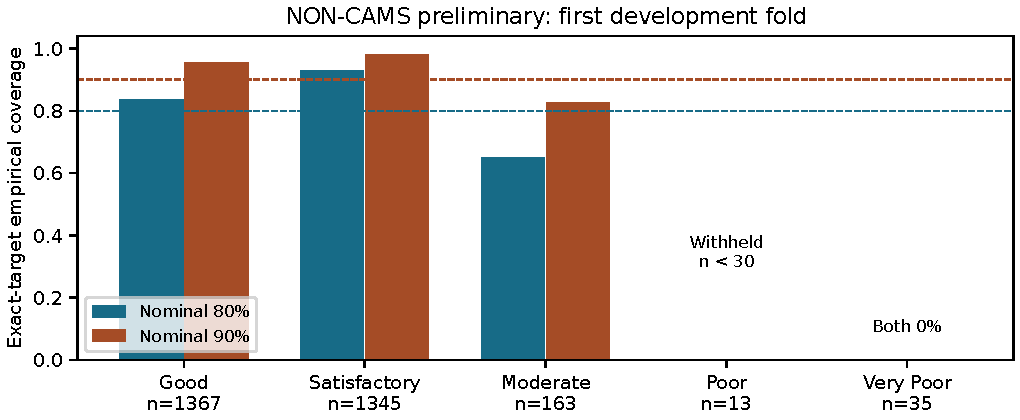
\includegraphics[width=\columnwidth]{../figures/coverage_vs_severity.pdf}
\caption{First-fold non-CAMS split-conformal coverage. Poor has only 13 exact pairs and its subgroup metric is withheld; Very Poor has 35. Neither constitutes primary CAMS evidence.}
\end{figure}
\begin{figure}[t]\centering
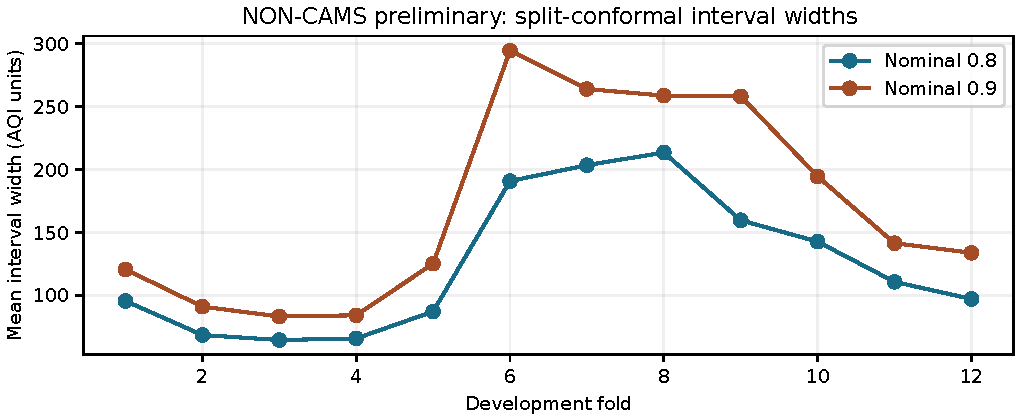
\includegraphics[width=\columnwidth]{../figures/interval_widths.pdf}
\caption{Mean interval widths across non-CAMS development folds, directly from the immutable result. These are fold summaries, not a manufactured distribution of individual interval widths.}
\end{figure}
\subsubsection{Interpretation of incomplete primary evidence}
Partial forecast extraction is an integrity milestone, not a forecast-skill
result. The current matched period cannot satisfy the 120-valid-day station
rule or the prescribed calibration and evaluation windows. The pipeline
therefore emits explicit insufficient-data entries rather than training on
a shorter interval. This affects all primary candidates, including raw CAMS,
climatology and persistence, so their intended paired comparison is not
quietly replaced by a convenient short-period leaderboard.

The non-CAMS result establishes that the experimental machinery can recover
differences against climatology, but the persistence comparison does not
establish an advantage for history Ridge. Likewise, near-nominal marginal
coverage can coexist with complete failure on a sufficiently supported
high-pollution subgroup. Those observations motivate the preregistered
severity and advisory analysis; they do not select a primary model. No
primary error scatter plot, error histogram or health-effect plot is supplied
because the required primary prediction artifacts do not yet exist.
